\section{GANDA (Choreographed Pair Performance) Category}
\label{sec:ganda_category}

            \begin{figure}[ht!]
            \centering
            \subfigure[]{\label{fig:ganda1}
                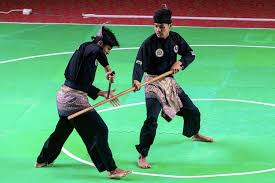
\includegraphics[height=1.5in]{images/ganda1}
            }
            ~
            \subfigure[]{\label{fig:ganda2}
                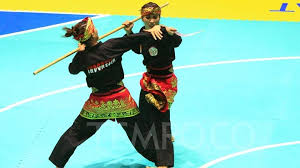
\includegraphics[height=1.5in]{images/ganda2}
            }
            \caption{Example Ganda Interactions}
            \label{fig:example_ganda}
            \end{figure}



\begin{legal}
\item Competition Equipment:


    \begin{legal}
    \item Attire: \\

    A standard Pencak Silat uniform (Figure~\ref{fig:tunggal_ganda_attire}) of any solid color (The top and bottom pieces may be of the same or different color) with a headband (a veil not covering the face, is not considered a headband) and `kain samping' of plain color or patterned. The color choice and combination are entirely at the discretion of the Contestant. It is allowed to have the badge of the contestant’s main association on the left chest and PERSILAT badge on the right chest. The national flag on the left arm and the name of the country at the upper back of the attire.

    \item Weapons:

        \begin{figure}[ht!]
        \centering
        \subfigure[Golok / Machete]{\label{fig:ganda_golok}
            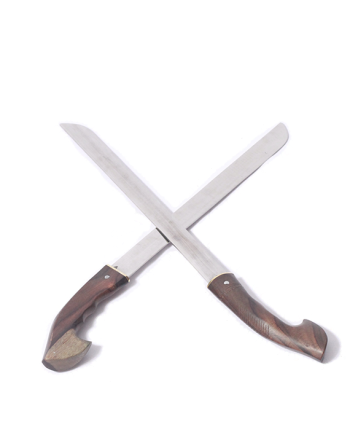
\includegraphics[height=2.5in]{images/golok}
        }
        ~
        \subfigure[Toya / Staff ]{\label{fig:ganda_toya}
            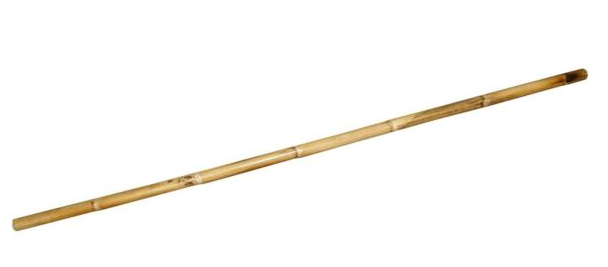
\includegraphics[height=1.5in]{images/toya}
        }
        \caption{Compulsory Weapons}
        \end{figure}

        \begin{figure}[ht!]
        \centering
        \subfigure[Keris]{\label{fig:ganda_keris}
            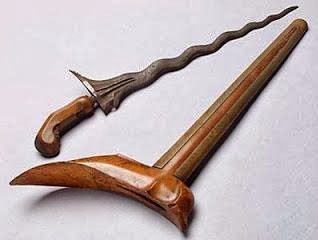
\includegraphics[height=2.5in]{images/keris}
        }
        ~
        \subfigure[Pisau / Knife]{\label{fig:ganda_pisau}
            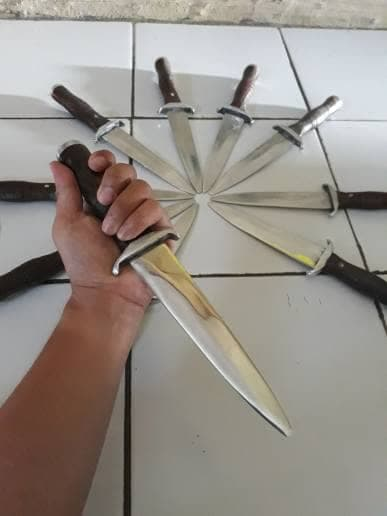
\includegraphics[height=2.5in]{images/pisau}
        }
        \subfigure[Clurit / Sickle]{\label{fig:ganda_clurit}
            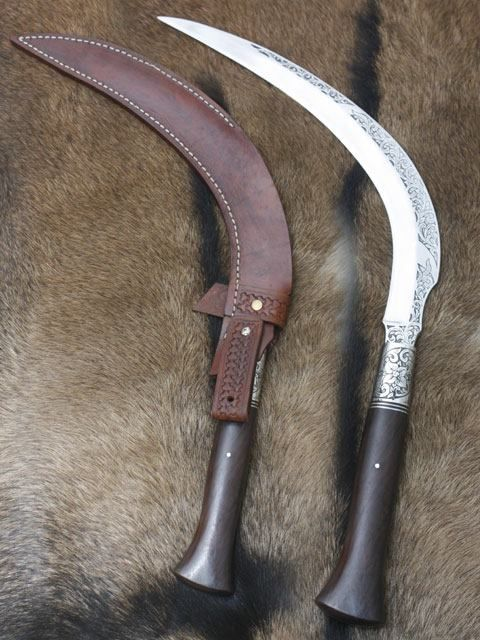
\includegraphics[height=2.5in]{images/clurit}
        }
        \subfigure[Trisula]{\label{fig:ganda_trisula}
            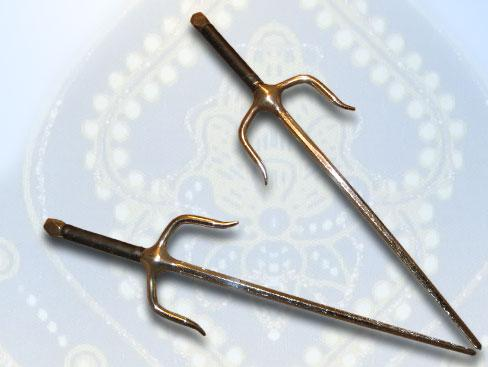
\includegraphics[height=2.5in]{images/trisula}
        }
        \caption{Selected Weapons}
        \end{figure}


        \begin{legal}
        \item The types, size and number of weapons to be used are as follows: \\ 
        
            Compulsory weapons: a golok/parang (short knife, Figure~\ref{fig:ganda_golok}) and 
            toya (long stick, Figure~\ref{fig:ganda_toya}) \\

            Selected weapons: It is compulsory to choose either one of these weapons: Keris (Figure~\ref{fig:ganda_keris}), 
            Pisau (knife, Figure~\ref{fig:ganda_pisau}), Clurit (sickle, Figure~\ref{fig:ganda_clurit}) and 
            Trisula (aka Cabang, Tekpi, Sai, Truncheon, Figure~\ref{fig:ganda_trisula}). \\

            The sequence of using compulsory and additional weapon is up to the discretion of the Pesilat.

        \item  For Senior, golok or parang is made of metal or wood, non-sharp pointed with length between 30 cm up 
               to 40 cm. With a width between 2.5 cm to 4 cm. Toya (long stick), made of rattan with the length of 
               between 150-180 cm and diameter of between 2.5-3.5 cm.

        \item For Junior, Senior and Master. (additional weapon)

            \begin{enumerate}[label=\alph*.]
            \item Knife made of metal or wood, non sharp-pointed with size between 15 cm up to 20 cm.
            \item Keris / sickle, sai made of metal or wood, non sharp-pointed with size between 30 cm up to 40 cm.
            \end{enumerate}

        \item The usage of selected weapon may be one or two pieces of a kind. Usage, technique and type of 
              selected weapons is up to the respective Silat Schools.

        \item The showcase is to begin as follows:
            \begin{enumerate}[label=\alph*.]
            \item To begin with bare-hand movement. \\
                  Free to continue:
            \item One Pesilat using weapon while the other bare-handedly, or both Pesilat using weapon.
            \item During performance the weapon moves (transfer) from one Pesilat to the other.
            \item Release or drop weapon in accordance with the performance description.
            \end{enumerate}

        \end{legal}



    \end{legal}
\item Competition Stages
    \begin{legal}
    \item When a competition is participated by more than 7 (seven) contestant, a pool system will be implemented.
    \item Three contestant with the highest scores from each pool will compete again in the next round. Unless the 
          following round is the final. \\
          The participants of the final round will be the best 3 (three) – in terms of gaining scores – from the 
          previous competition pool stages.
    \item The number of pools is decided in a meeting attended by the International Technical Delegates, Competition 
          Chairperson and Council of Jury. The decision will be announced to the participants at the Technical Meeting.
    \item The pool division for contestants are determined by drawing of lots during the Technical Meeting. Voting method, i.e either manually or digitally will be decided through voting at the Technical Meeting.
    \item Each category should be participated by minimum 2 (two) participants and directly goes to final round.
    \end{legal}

\item Duration of Competition \\

      The performance duration is 3 (three) minutes.

\item Competition Procedure
    \begin{legal}
    \item The beginning of competition:
        \begin{enumerate}[label=\alph*.]
        \item Juries reporting for duty to the Competition Chairperson from the right side of the 
              Competition Chairperson
        \item how respect and readiness to perform duty
        \item Taking the allocated seats
        \end{enumerate}

    \item The weapons that were certified by the Competition Chairperson will be placed at the weapon quarantine station as prepared by the organizing committee. Pesilat/coach will be allowed to collect the weapons just before he/she enter the arena (immediately after his/her name was announced).

    \item Pesilat
        \begin{enumerate}[label=\alph*.]
        \item Entering the arena from the left side of the Competition Chairperson
        \item Walk towards the centre of arena
        \item Pesilat is to place the weapon on the mat (no assistance from coach)
        \item Show respect to the Competition Chairperson and turning back to show respect to the Jury committee.
        \end{enumerate}

    \item Competition Chairperson will signal the Juries, time keeper and other Competition official to alert them that duty is about to begin.

    \item The showcase
        \begin{enumerate}[label=\alph*.]
        \item Showcase the Opening PERSILAT greeting
        \item The gong will be stricken to mark the beginning of performance time
        \item Pesilat will perform the showcase
        \item The gong will be stricken to mark the end of performing time
        \end{enumerate}

    \item At the end of the performance
        \begin{enumerate}[label=\alph*.]
        \item Contestant to show respect to the Juries and Competition Chairperson from the center of the arena
        \item To leave the arena by the left side of the Competition Chairperson
        \end{enumerate}

    \item Time Keeping
        \begin{enumerate}[label=\alph*.]
        \item The Competition Chairperson will make sure/take charge of the showcase time
        \item The Time Keeper will keep track of the 3 minutes showcase
        \item Competition Chairperson will announce the actual showcase time. (If digital scoring is used, 
              the time tracking will be as displayed on the screen)
        \end{enumerate}

    \end{legal}


\item Competition Rules
    \begin{legal}
    \item Rules of the game
        \begin{legal}
        \item For 3 (three) minutes the participant performs the richness technique of jurus attack-defense with bare hands and with weapons.\\
        A tolerance period of +/-5 seconds is allowed.\\
        Should the tolerance period go beyond the limit, penalty will be imposed accordingly.
        \item Uttering of sound is allowed
        \end{legal}

    \item Penalties
        \begin{legal}
        \item\label{pt:ganda_deductions} Deduction of score is imposed each time contestant performs the following faulty:
            \begin{enumerate}[label=\alph*.]
            \item\label{pt:ganda_time_factor} Time Factor
                \begin{enumerate}[label*=\arabic*.]
                \item Beyond the tolerance period
                    \begin{enumerate}[label*=\arabic*.]
                    \item five (5) to ten (10) seconds deduction. Should the showcase go beyond these tolerance 
                    period the showcase will be stopped and declared disqualified.
                    \end{enumerate}
                \item Other factors \\
                    Deduction of 5 (five) points penalty will be imposed to the following:

                    \begin{enumerate}[label=\roman*.]
                    \item Contestant crosses the arena borderline (10m x 10m)
                    \item Each time the weapon drop against prescription
                    \item Weapon did not drop as prescribe in the prescription
                    \item The weapons that was prescribe as drop (in the prescription), drop outside
                        the arena and pesilat crosses the arena to pick the weapon (as it is still needed
                        for the showcase)
                    \item using not fully proper weapon according to the regulation, or broken golok,
                        broken toya, golok loose from its head.
                    \end{enumerate}
                
                \end{enumerate}
            No deduction of score for accessories falls.
            \end{enumerate}
        \item Walk-Out \\
        Participation will be declared as Walk-out should the contestant fail to report to the Competition’s 
        Secretary after being call for the 3rd time.\\

        The interval between the call outs will be at thirty (30) seconds each.

        \item Disqualification
            A Pesilt will be disqualified for:
            \begin{enumerate}[label=\alph*.]
            \item Wearing a non-compliant uniform 
            \item Using a weapon not allowed by competition regulations 
            \item Violating time limits as stated in point~\ref{pt:ganda_deductions}~\ref{pt:ganda_time_factor}.
            \item Being unable to show the letter of medical health before the start of competition 
            \end{enumerate}

        \end{legal}

    \end{legal}

\item Scoring
    \begin{legal}
    \item Scoring consist of:
        \begin{legal}
        \item Score of attack-defense technique:\\
            The score of attack-defense technique – bare-handed or armed, includes various attack-defense 
            techniques by hands or foot such as: hitting, kicking, sweeping, dropping, parrying, 
            dodging/evading, catching, locking, etc.

        Scoring shall focus on the following elements:

        \begin{enumerate}[label=\alph*.]
        \item The quality of attack-defense techniques in barehanded as well as using weapon.
        \item The richness of attack-defense techniques in barehanded as well as using weapon.
        \item The skill and creativity of attack-defense techniques
        \item The logic in executing attack-defense technique
        \end{enumerate}

        Score ranges from 60 (sixty) to 80 (eighty) points which is the total score of the above four elements of technique.

        \item Firmness Score: \\
        Firmness score consists of elements of firmness, harmony, courage of both Pesilats during performance.

        Scoring shall focus on the following elements:

            \begin{enumerate}[label=\alph*.]
            \item Firmness and strictness of movement
            \item Harmony/solidity of both Pesilats
            \item Courage in weapon skill
            \item Power and stamina
            \end{enumerate}

        Score ranges from 50 to 60 points which is the integrated score of the above four elements of firmness.

        \item Soulfulness score includes the following elements:
            \begin{enumerate}[label=\alph*.]
            \item The harmony of expression of movement soulfulness
            \item The harmony of movement rhythm score ranges from 50 (fifty) to 60 (sixty)
                  points which is the integrated score of both elements of soulfulness. 
            \end{enumerate}
        \end{legal}
    \end{legal}

\item Decision and announcement of the winner
    \begin{legal}
    \item\label{pt:ganda_winner} The winner is the contestant who gains the highest score for his/her performance from 3 (three) out of 5 (five) jurors with elimination of the highest and the lowest score.
    \item If the scores are equal, the winner will be determine accordingly:
            \begin{enumerate}[label=\alph*.]
            \item The contestant who gains the total highest Technique points from the 3 (three) jurors as decided in para~\ref{pt:ganda_winner}
            \item The contestant who gains the highest points in firmness, soulfulness and stamina from 3 (three) jurors as decided in para~\ref{pt:ganda_winner}
            \item  The contestant whose duration of performance is the closest to precise time of 3 (three) minutes.
            \item  The winner is the contestant who gains the least penalty points.
            \item If the result remains the same,the Competition Chairperson will do a coin toss on to the mat 
            witnessed by Technical Delegate, Council of Juror and Team Managers of respective contestant. 
            \end{enumerate}
    \item The score of each contestant is announced after the Jury has finished their task in giving score to all contestant of the category.\\

    Total scores will be shown on the scoreboard while announced by the Competition Chairperson except when using a digital scoreboard where the scores from each Jury and total scores are displayed in the screen instantly.

    \end{legal}

\end{legal}
